%%%%%%%%%%%%%%%%%%%%%%%%%%%%%%%%%%%%%%%%%%%%%%%%%%%%%%%%%%%%%%%%%%%%%%%%%%%%%%%%%%%
\documentclass[12pt,oneside]{article}
\usepackage{geometry}
\usepackage[table,xcdraw]{xcolor}
\usepackage{float}
\usepackage{wrapfig}
\usepackage{graphicx}
\usepackage{subfigure}
\usepackage[table,xcdraw]{xcolor}
\usepackage{amsmath,amssymb,amsfonts,amscd, array,amsthm}
\geometry{verbose,tmargin=1in,bmargin=1in,lmargin=1in,rmargin=1in}
\usepackage{rotating}
\usepackage{pdflscape}
\begin{document}
\begin{titlepage}
	\centering
	{\huge\bfseries Characterization and Validation of a Precursor Drawn Monofilament for Twisted Polymer Actuators and Free Torsion Actuation Data\par}
	\vspace{1cm}
	{\scshape\LARGE by\par}
	\vspace{1cm}
	{\LARGE\itshape Diego Ricardo Higueras Ruiz\par}
	\vspace{1cm}
	{\large advised by: Dr.~Michael Shafer $\&$ Dr. Heidi Feigenbaum\par}
	\vspace{2cm}
	{\large\bfseries A THESIS PROPOSAL SUBMITTED IN PARTIAL FULFILLMENT OF THE REQUIREMENTS FOR THE DEGREE OF \par}
	\vspace{0.5cm}
	{\large\bfseries MASTERS OF APPLIED SCIENCE \par}
	{\large\bfseries in the school of Mechanical Engineering \par}
	\vspace{0.5cm}
	{\large\bfseries NORTHERN ARIZONA UNIVERSITY \par}
	\vspace{2cm}
	{\LARGE \today\par}
	\vfill
	% Bottom of the page
	{\large\bfseries All rights reserved. This work may not be \\ reproduced in whole or in part, by photocopy \\ or other means, without the permission of the author. \par}
	
\end{titlepage}

%%%%%%%%%%%%%%%%%%%%%%%%%%%%%%%%%%%%%%%%%%%%%%%%%%%%%%%%%%%%%%%%%%%%%%%%%%%%%%
\section*{Introduction to Research Topic}
	\hspace{0.4cm}It was recently shown that drawn polymer monofilaments, such as Nylon fishing line have the ability to supply linear actuation when it is configured as a coil Twisted-coiled Polymer Actuator (TCPA) [8]. However, it has not been clearly explained what the primary driving mechanism of these axial actuators is. Dr. Ray Baughman and his team at the University of Texas in Dallas [8] claim that axial actuation in TCPAs is caused by anisotropic thermal expansion in the radial and axial directions. Since, no clear explanation has been presented, suggesting no final demonstration has been achieved.\par	
	
	In the interest of achieving a suitable model for nylon actuators, our team has looked toward understanding how twisted nylon fibers react when a temperature gradient is applied. Here we present the straight twisted polymer actuator (STPA), which is a precursor fiber that is twisted about
its central axis but still remains straight. Even though the twisted precursor remains straight, after the twisting process of manufacture, the polymer chains will be helically oriented about the central axis.\par 

	We consider this configuration the first step to take in order to
model more complex nylon actuator configurations as TCPAs. So far, two models have been presented for STPAs: Shafer's [4] and Aziz's [9] model. These two models use the thermo-mechanical properties of the precursor fiber to predict torsional actuation. The purpose of this thesis is to characterize the thermo-mechanical properties of the precursor fiber and obtain accurate prediction by using the two mentioned models of torsional actuation under no load. This work also involves the process of experimentally validating the model and properties to ensure its accuracy.

	


	
	  

%%%%%%%%%%%%%%%%%%%%%%%%%%%%%%%%%%%%%%%%%%%%%%%%%%%%%%%%%%%%%%%%%%%%%%%%%%%%%%
\section*{Objectives}

%\subsection*{-Dynamic and Active Systems Laboratory (DASL) Objetives}
%\begin{enumerate}
%	\item Characterization of the thermo-mechanical properties of the 				precursor drawn monofilament of Nylon 6.6 with the brand name of "Berkley 		SUPER STRONG TRILENE" of Twisted Polymer Actuators.
%	\item Compare experimental torsional actuation of a Twisted Polymer 			Actuator under no load using the previous found properties in the Shafer's 	and AZIZ mathematical models. 
%\end{enumerate} 

\subsection*{-Thesis Objectives}
\begin{enumerate}
	\item Complete a literature review on the body of the work on 		smart axial and torsional actuation, as well as a review on the material 		modeling of mechanical properties and behavior of the precursor material.
	\item Qualitative and quantitative characterization of the precursor 			material known as drawn monofilament of Nylon 6.6 with the brand name of ``Berkley Super Strong Trilene'' as a function of the variables, which play an important role in 		the mechanism of actuation of Twisted Polymer Actuators, including its 			elastic and viscoelastic behavior. The following properties must be 			studied in depth to fully predict the actuation of TPAs:
	
	\begin{itemize}
	 		\item Axial modulus as a function of temperature
			\item Radial modulus as a function of temperature
			\item Shear modulus as a function of temperature
			\item Poisson ratio
			\item Thermal axial contraction
			\item Thermal radial expansion
	\end{itemize}
	\item Compare experimental torsional actuation of a Twisted Polymer 			Actuator under no load with the previous found properties by using the Shafer's 	and Aziz's mathematical models. 	
\end{enumerate}


\section*{Relevance to this Field}

\subsection*{Torsional actuation with Smart Materials}
\hspace{0.4cm}Many different smart materials have been studied to create torsional actuation. Some renowned smart materials in this engineering field are CNT (Carbon Nanotube), SMA (Shape Memories Alloys), EAP (Electroactive Polymers) and SMP (Shape Memory Polymer), and the one study here, STPA (Straight Twisted Polymer Actuators). However, other non-smart materials but innovative torsional actuators can be mentioned like PAMs (Pneumatic Torsional Actuators) and HAMs (Hydraulic Actuators). \par
 All of these smart materials are unique in behavior and properties. The mechanism of activation differs from one type to other due to the coupling that occurs between different fields of the materials (electric, magnetic or thermal field), in the case of STPAs there is a thermo-mechanical coupling, which is the driving force of actuation. \par 
 All of these materials can play similar roles in torsional actuation, but the affordability of STPAs is an aspect to highlight, this feature put nylon actuators in a competitive position regard the rest of the smart material on the market. \par
 The features table 1 has been attached to this proposal to give a better understanding of the main actuation properties to study in torsional actuation, as well as provide a comparison between the different current technologies in this field.

% Please add the following required packages to your document preamble:

% If you use beamer only pass "xcolor=table" option, i.e. \documentclass[xcolor=table]{beamer}
\vspace{3.55cm}
\begin{table}[]
\vspace{-3.55cm}

\centering
\small
\caption{Main features of torsional actuators}
\vspace{1cm}
\label{my-label}
\begin{tabular}{
>{\columncolor[HTML]{C0C0C0}}c cccccc}
\cellcolor[HTML]{9B9B9B}\textbf{Ref.}                & \cellcolor[HTML]{9B9B9B}\textbf{\begin{tabular}[c]{@{}c@{}}Type of \\ Torsional \\ Actuator\end{tabular}} & \cellcolor[HTML]{9B9B9B}\textbf{\begin{tabular}[c]{@{}c@{}}Activation \\ Mechanism\end{tabular}} & \cellcolor[HTML]{9B9B9B}\textbf{\begin{tabular}[c]{@{}c@{}}Specific\\ gravity\end{tabular}} & \cellcolor[HTML]{9B9B9B}\textbf{\begin{tabular}[c]{@{}c@{}}Free\\ torsion.\\ \begin{small}($\dfrac{\circ}{mm}$)\end{small}\end{tabular}} & \cellcolor[HTML]{9B9B9B}\textbf{\begin{tabular}[c]{@{}c@{}}Torque \\ normalized \\ by cross \\ sectional\\ \begin{small}($\dfrac{N}{mm^2}$)\end{small}\end{tabular}} & \cellcolor[HTML]{9B9B9B}\textbf{\begin{tabular}[c]{@{}c@{}}Magnitude of \\ activation\end{tabular}} \\\\

{[}1,2{]}                                            & CNT                                                                                                       & Temperature                                                                                      & 1.6                                                                                         & 15 $\sim$ 80                                                                                     & 0.5 $\sim$ 1.8                                                                                                            & 0 $\sim$ 90$^{\circ}$C                                                                                      \\\\
{[}3{]}                                             & SMA                                                                                                       & Temperature                                                                                      & 6.5                                                                                         & 0.18                                                                                             & 100 $\sim$ 200                                                                                                            & 0 $\sim$ 100$^{\circ}$C                                                                                     \\\\
{[}4{]}                                             & STPA                                                                                                       & Temperature                                                                                      & 1.12                                                                                        & $\sim$12.7                                                                                       & 0 $\sim$ 119                                                                                                              & 0 $\sim$ 90$^{\circ}$C                                                                                      \\\\
{[}5{]}                                             & \begin{tabular}[c]{@{}c@{}}EAPs\\ Ion-based \\ actuation\end{tabular}                                     & Electricity                                                                                      & 1.12                                                                                        & 0.01                                                                                             & N/A                                                                                                                       & \begin{tabular}[c]{@{}c@{}}0 $\sim$ 4 V\\ (Alternating \\ Current)\end{tabular}                     \\\\
{[}6{]}                                             & \begin{tabular}[c]{@{}c@{}}PAMs\\ (Antagonistic \\ Torsion Shape \\ Actuators)\end{tabular}               & \begin{tabular}[c]{@{}c@{}}Pneumatic\\ (Pressure)\end{tabular}                                   & ...                                                                                           & 0.287                                                                                            & 0 $\sim$ 1.43                                                                                                             & 50 $\sim$ 90 kPa                                                                                    \\\\
{[}7{]}                                             & \begin{tabular}[c]{@{}c@{}}PAMs\\ (Peano \\ Actuators)\end{tabular}                                       & \begin{tabular}[c]{@{}c@{}}Pneumatic\\ (Pressure)\end{tabular}                                   & ...                                                                                           & 0.315                                                                                            & 0 $\sim$ 0.713                                                                                                            & 50 $\sim$ 90 kPa                                                                                    \\\\
\multicolumn{1}{l}{\cellcolor[HTML]{C0C0C0}{ [}8{]}} & \begin{tabular}[c]{@{}c@{}}SMP\\ Shape Memory\\ Polymers\end{tabular}                                     & Temperature                                                                                      & 1.12                                                                                        & $\sim$1.8                                                                                        & $\sim$1                                                                                                                   & 0 $\sim$ 62$^{\circ}$C                                                                                      \\\\
\multicolumn{1}{l}{\cellcolor[HTML]{C0C0C0}N/A}      & HAMS                                                                                                      & Hydraulic                                                                                        & N/A                                                                                         & N/A                                                                                              & N/A                                                                                                                       & N/A                                                                                                
\end{tabular}
\end{table}
\newpage
\subsection*{Characterization of a Precursor Drawn Monofilament of Nylon 6.6}

 \hspace{0.4cm}In terms of free torsional displacement actuation only two properties of the precursor fiber are required; axial and radial thermal expansion. However, for other actuation scenarios where a load is involved, the rest of properties will play a role in the equation of actuation.
 
 In the characterization of a material mechanical properties there are a couple of considerations that are key in order to obtain reliable properties. In this respect, we consider the precursor fiber a transversely isotropic material, where the material is perfectly characterized by finding the properties in the radial and axial directions.\par

 Another aspect to consider is how the material is going to behave when stresses are applied. Two different behaviors are studied in this thesis: Linear elasticity and viscoelasticity. It is worth mentioning that linear elastic behavior (Hooke's Law) is easier to model than viscoelastic behavior; nonetheless, we will state when elastic behavior is a great approximation under certain circumstances.\par
\vspace{0.5cm}
\hspace{0.4cm} \textbf{Linear Elastic Behavior} \par 
\vspace{0.5cm}
	In this section, the 3D stress-strain relationships for transversely isotropic materials will be considered within a linear range.
	
\begin{figure}[H]
\centering	
\vspace*{-2cm}
	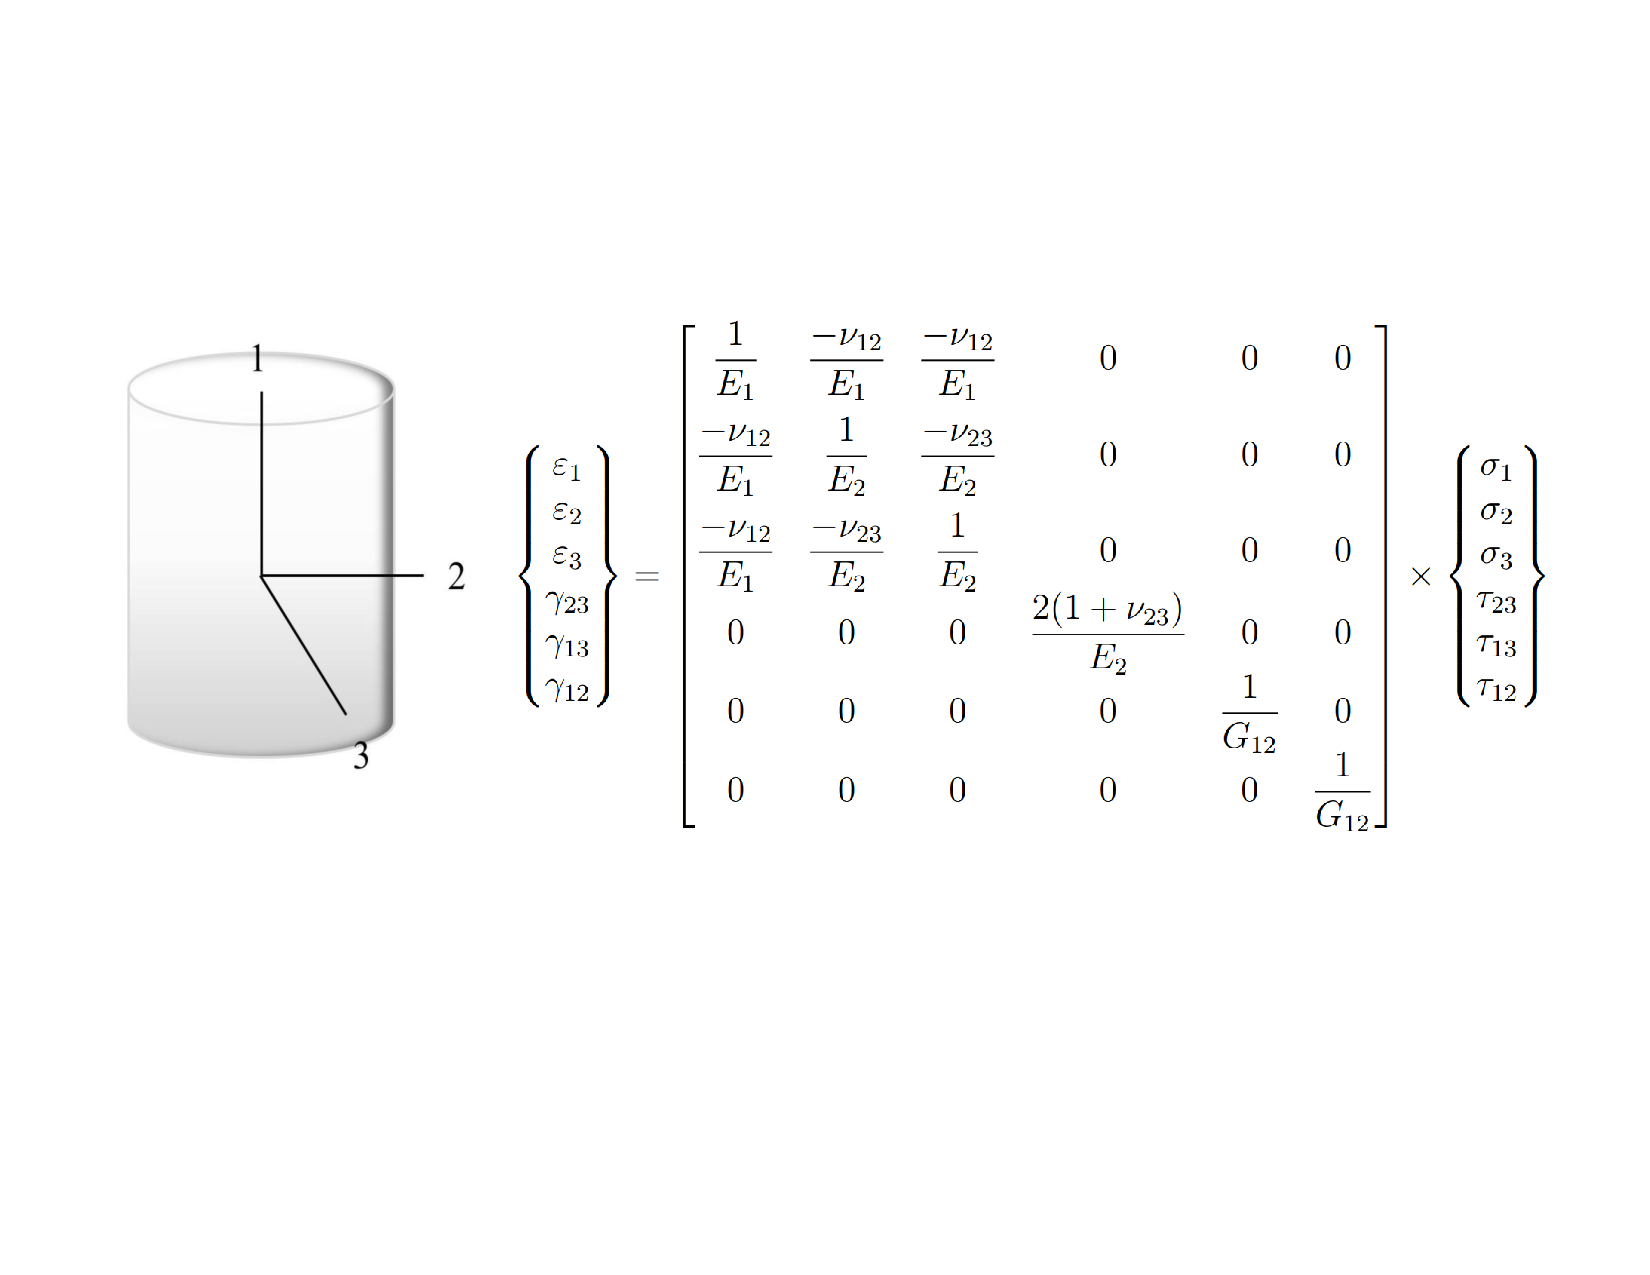
\includegraphics[width=17cm,height=12cm, angle=0]{transisotropicicmatrix.pdf}
\vspace*{-4cm}
\caption{Transversely Isotropic Compliance Matrix.}\label{fig:precursorfiberwithcoordsystem}
\end{figure}
Illustration 1 shows a transversely isotropic material. Configuration, where the 2 and 3 axis (radial directions) are assumed to be planes of isotropy. Thus all properties in the radials directions are going to be the same. This fact can be translated to the compliance matrix that is well defined with only five independent variables. \par
\vspace{0.5cm}
\textbf{Viscoelasctic Elastic Behavior} \par 
\vspace{0.5cm}
 Most of the polymers materials exhibit a combination of elastic and viscous responses when external loads and deformations are applied. This behavior is more complicated than Hookean solids. Some models that have been studied are: Boltzman superposition, spring-dashpot configurations or complex modulus notation model. In this thesis we will work through these models and obtain the closest fit for the precursor fiber. 




\subsection*{Validation of Shafer's and Aziz's Model with the Obtained Properties using Experimental Results}

\hspace{0.5cm}The models that have been presented in journal articles so far are the Shafer's model in the DASL at the Northern Arizona University and Aziz's model at the University of Wollogon. These are the model that we are going to be testing for validation. \\ \par

\hspace{0.5cm}\textbf{Shafer's Model}\\ \par

This model predicts the free rotation of a STPA as a function of thermal load under the main assumptions of: considering the precursor monofilament a transversaly isotropic linear-elastic material, constant pitch angle as a function of the radius, and the fibers at each raddi are free to expand/contract due to thermal loading without stress. \par
	The model uses precursor drawn fiber axial thermal expansion, $\varepsilon^{t}_{11}$, and the radial thermal expansion, $\varepsilon^{t}_{22}$ to predict the untwist ($\Delta \phi$) and change in length ($L_f - L$) of the polymer monofillament under thermal loads.\par 

	This model is based on a transformation of coordinate system of the chain polymer (1 $\&$ 2 directions) to the radial (r), tangential ($\theta$), and axial (z) coordinates direction by using the pitch angle. As a matter of simplification a non-dimensional initial twist; $x = \dfrac{r \phi_o}{L}$, is defined where "r" is the radial position of a particular fiber, $\phi_o$ is the initial twist into the fiber, and L the initial length of the monofilament. 
	
\begin{figure}[H]
\centering	
	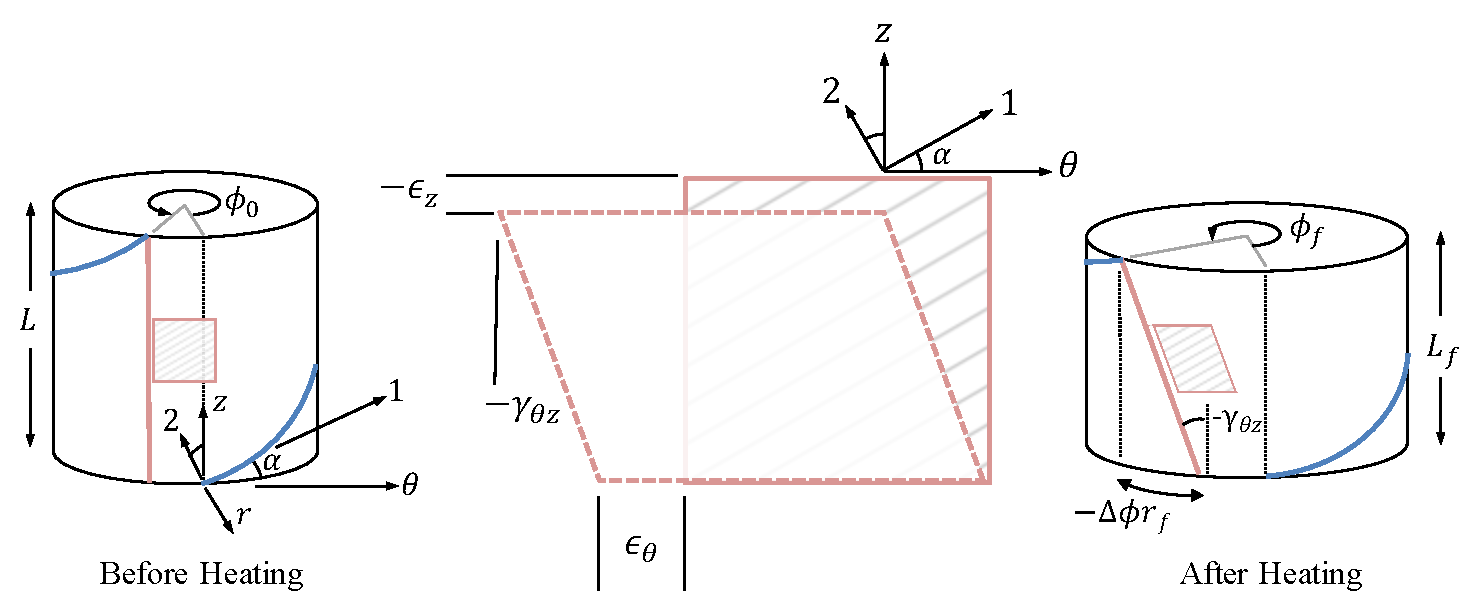
\includegraphics[width=15cm,height=6cm, angle=0]{elemental_diagram_2.pdf}
	
\caption{Transition of a STPA under thermal load with principal and converted coordinate systems.}\label{fig:aaa}
\end{figure}	
	 	
	
	As a result of this coordinate transformation and simplifications, the change in length can be predicted as the equation 1 shows:
	
	\begin{equation}
\Delta L = L_f - L = \varepsilon^t_{z} L = \frac{\varepsilon^{t}_{22} x^2 + \varepsilon^{t}_{11}}{1+x^2} L
\label{eq:DL}
\end{equation} 	

 And the change in untwist can be calculated as the equation 2 shows:
 
 \begin{equation}
%\Delta \phi = \frac{[(1+\varepsilon^{t}_{11})+ (1+\varepsilon^{t}_{22})x^2]L}{[(1+\varepsilon^{t}_{22})+ (1+\varepsilon^{t}_{11})x^2]r} \tan \gamma^t_{z \theta}
\frac{\Delta \phi}{\phi_0} = \frac{(\varepsilon^{t}_{11}-\varepsilon^{t}_{22})}{1+x^2}
\label{eq:Dphi}
\end{equation} 	
 	
%% AZIZ MODEL
\hspace{0.5cm}\textbf{Aziz's Model}\\ \par

Another model has been presented, where torsional actuation is attributed to the radial thermal expansion. This model neglects changes in length in the axial direction and is not valid for temperatures in the range of 26 to 62 $^\circ C$. In this model the torsional stroke in turns for fiber length was claimed to be $\Delta T$ :

 \begin{equation}
 \Delta T = \frac{n_o}{l_o}(\frac{d_o}{d}-1)
\label{eq:aziz_mod_T}
\end{equation}

In the equation 3, $n_o$ is the initial number of twists, $d_o$ is the initial fiber diameter, $l_o$ length of the fiber, and $d$ is the fiber diameter as a function of temperature.

Equation 3 can be converted in terms of untwist in radians ($\Delta \phi$) and the radial thermal expansion ($\varepsilon^{t}_{22}$) in order to be able to analyze a general case. The prediction of the untwist fiber is given by $\Delta \phi$ in radians, in the equation 4:
\begin{equation}
\Delta \phi = -\phi_o \frac{\varepsilon^{t}_{22}}{\varepsilon^{t}_{22}+1} 
\label{eq:aziz_mod_e22}
\end{equation}

where $\phi_o$ is the initial twist in radians.

%\begin{figure}[ht]
%\centering
%\includegraphics[width=0.95\textwidth]{Aziz_diagram}
%\caption{Aziz et al. model diagram.}
%\label{fig:Aziz}
%\end{figure}	 

	


\subsection*{Completed Work}
\hspace{0.4cm} A complete literature review and characterization of nylon actuators will be submitted as a part of this thesis work, as well as an analysis of the microstructure of drawn monofilament of nylon 6.6.\par


An assessment of the obtained properties in the models will be presented and experimentally validated. To date, no reliable properties of the precursor fiber of nylon 6.6 have been published and this is a crucial work that need to be done in order to predict the actuation of STPAs. For this reason, in this work the properties of the precursor fiber will be found as a  function of temperature. In addition, an study of the behavior of the precursor material will be done in order to analyze how the monofilament performs as a function of temperature or other parameters that might be critical in the characterization process. \par

Finally, we will use the obtained results to predict the actuation of STPAs with different numbers of inserted twists to see how they perform as a function of the pitch angle and validate these results with experimental data.



\subsection*{Time Line}
\begin{figure}[H]
\hspace{-4cm}
	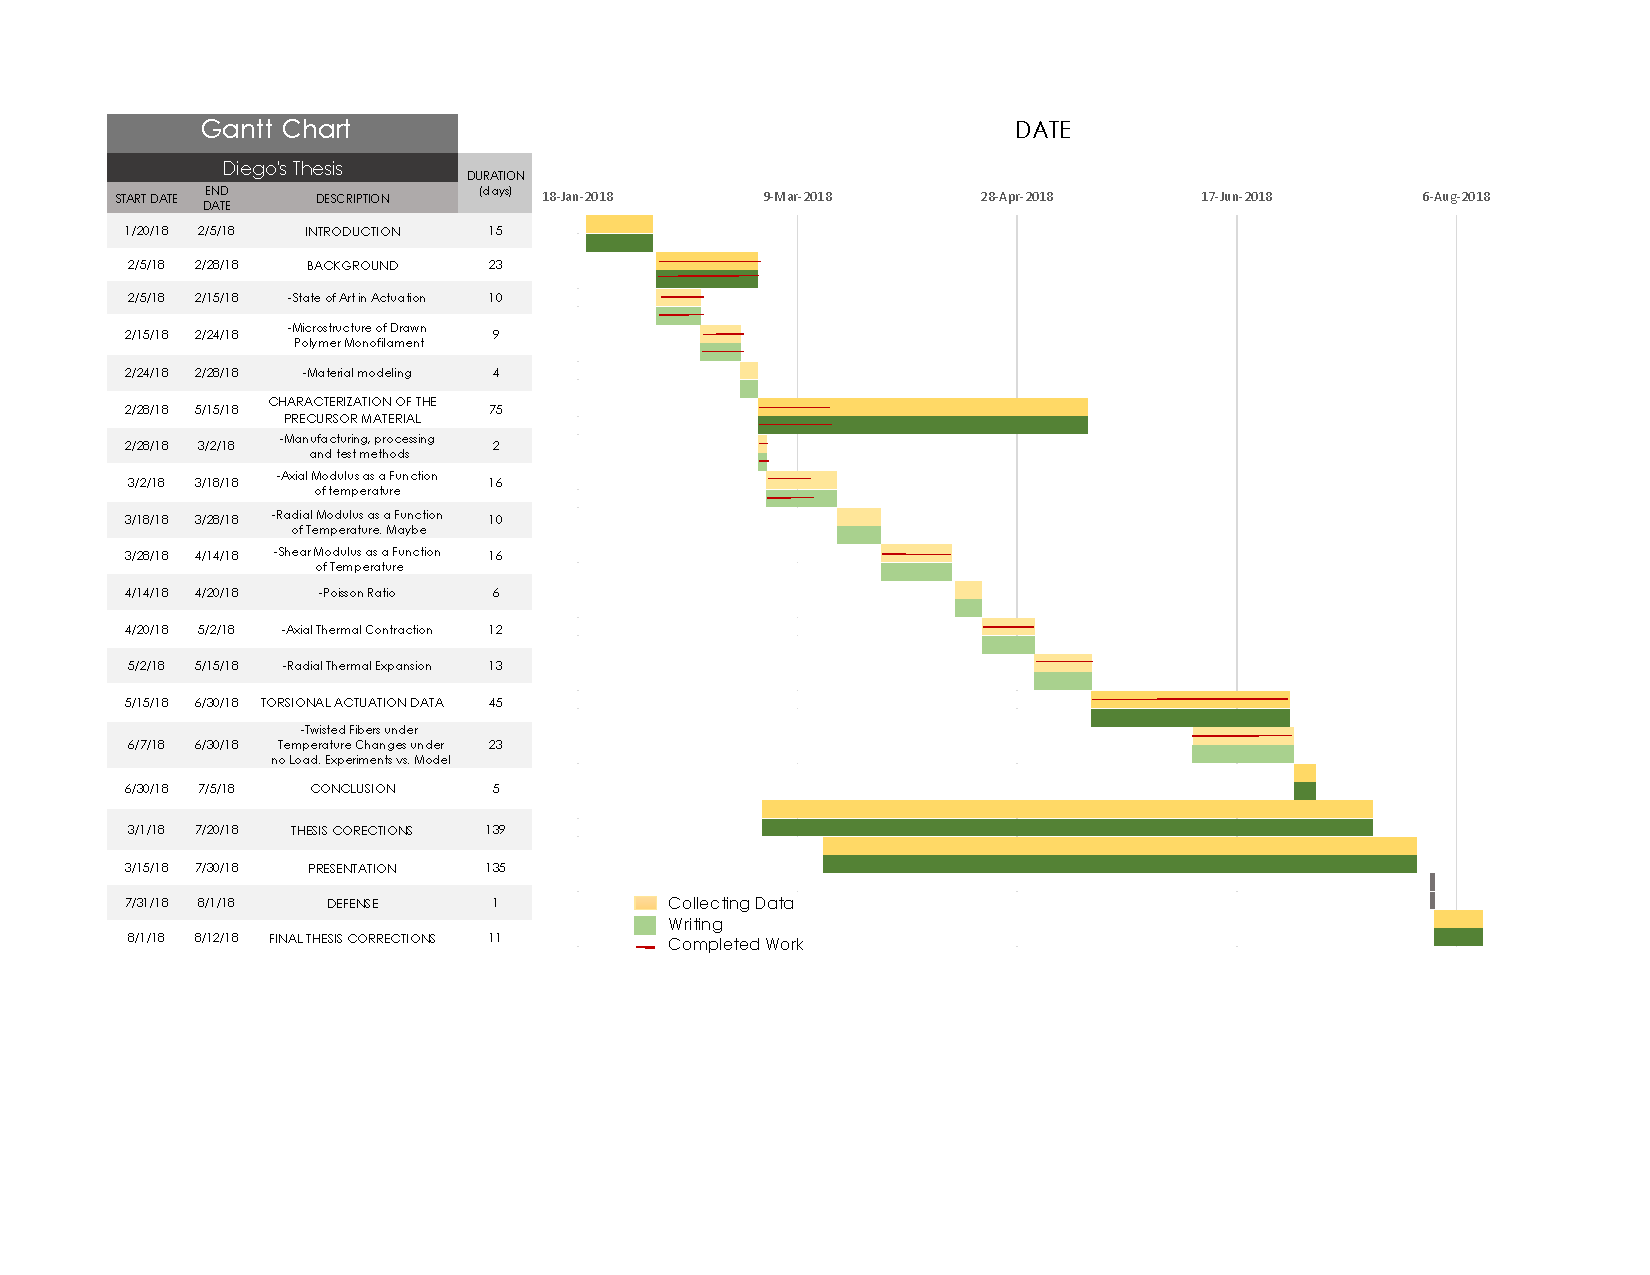
\includegraphics[clip,trim=1.8cm 0 0 1.4cm,width=24cm,height=19cm, angle=-90]{finalganttchart.pdf}
\caption{Time line}\label{fig:Time line}
\end{figure}



\subsection*{Future Work}
\hspace{0.4cm} After the characterization of the precursor material and modeling of the actuation under no load, the model will be expanded to account for actuation with applied loads, being this case that will be presented in real life applications. This upgraded model will predict torsional stroke and developed torque as a function of temperature. \par 

	In terms of modeling, a new model could be created for predicting the actuation of axial nylon actuators. This is considered the most complex model; nevertheless, it is expected for this model will follow the same principles of torsional actuators models.\par 

	After characterization and modeling of the material, implementation is the final step. Different type of configurations can be built in order to create different applications. In implementation, activation method is another topic to consider, since more of the efficiency drop is due to thermal losses between the thermal source and the nylon actuator. 



\subsection*{References}

\hspace{.5cm}
 [1] Dongseok Suh, Thuy Kieu Truong, Daniel G. Suh,  and Seong Chu Lim. 2016.”Torsional Actuator Powered by Environmental Energy Harvesting from Diurnal Temperature Variation”. Department of Energy Science, Sungkyunkwan University, Suwon 16419, Korea. The Alan G. MacDiarmid NanoTech Institute, University of Texas at Dallas, Richardson, Texas 75083, United States. ACS Sustainable Chem. Eng., 4 (12), DOI: 10.1021/acssuschemeng.6b01502 pp 6647–6652. \par
\vspace{0.4cm}

[2] Kyoung-Yong Chun, Shi Hyeong Kim, Min Kyoon Shin, Cheong Hoon Kwon, Jihwang Park, Youn Tae Kim, Geoffrey M. Spinks, Marcio D. Lima, Carter S. Haines, Ray H. Baughman and Seon Jeong Kim. 2013. "Hybrid carbon nanotube yarn artificial muscle inspired by spider dragline silk". Nature Communications. 5:3322 | DOI: 10.1038. pp 1-9.\par
\vspace{0.4cm}
[3]. A. Peter Jardine, Jayanth N. Kudva, Christopher Martin and Kari Appa, Northrop-Grumman Corp. 1996. Shape Memory Alloy TiNi “Actuators for Twist Control of Smart Wing Designs”. pp 1-6.\par
\vspace{0.4cm}
[4] Michael W. Shafer, Heidi P. Feigenbaum, Daniel Pugh and Matthew Fisher. 2016. "First steps in modeling thermal Actuation of Twisted Polymer Actuators using virgin material properties". SMASIS2016-9292. pp. 1-9.\par
\vspace{0.4cm}
[5] Yang Fang, IEEE Member,Thomas J. Pence, and Xiaobo Tan, IEEE Member. 2011. “Fiber-Directed Conjugated-Polymer Torsional Actuator: Nonlinear Elasticity Modeling and Experimental Validation”. IEEE/ASME TRANSACTIONS ON MECHATRONICS, VOL. 16, NO. 4. pp 656-667.\par
\vspace{0.4cm}
[6] Siddharth Sanan Peter S. Lynn Saul T. Griffith. Carnegie Mellon University]. 2013. “Pneumatic Torsional Actuators for Inflatable Robots”. PhD Thesis.  pp 1-9\par
\vspace{0.4cm}
[7]. M. Baghani. School of Mechanical Engineering, College of Engineering, University of Tehran. 2017. “Analytical study on torsion of shape-memory-polymer prismatic bars with rectangular cross-sections”. International Journal of Engineering Science 76 (2014) pp 1–11. \par
\vspace{0.4cm}
[8] Carter S. Haines et al. 2014. Artificial Muscles from Fishing Line and Sewing Thread.  DOI. 10.1126/science.1246906 Science 343, pp 868 - 872.\par
\vspace{0.4cm} 
[9] Shazed Aziz, Sina Naficy, Javad Foroughi, Hugh R. Brown, Geoffrey M. Spinks. 2016. Controlled and Scalable Torsional Actuation of Twisted Nylon 6 Fiber. University of Wollongong. pp1278-1286. \par


\end{document}
